\section{Results}\label{sec:results}

\subsection{Dense Physical Graphs and Oversmoothing}\label{sec:oversmoothing}

A fundamental finding across our experiments is that dense physical graphs degrade T-GCN performance. Table~\ref{tab:oversmoothing} compares the physical graph against a no-graph baseline and sparse learned graphs, all on Los-loop (PH=1, seed=42).

\begin{table}[t]
\centering
\caption{Oversmoothing evidence: Los-loop (PH=1, seed=42). Dense graphs---whether physical or learned from correlations---produce substantially worse RMSE than no graph at all, isolating density (not the graph's origin) as the harmful factor. Sparse learned graphs and multi-lag graphs improve over T-GCN-NoSpatial.}
\label{tab:oversmoothing}
\begin{tabular}{lccc}
\toprule
\textbf{Graph} & \textbf{Edges} & \textbf{RMSE} & \textbf{MAE} \\
\midrule
Physical (207 nodes) & 2833 & 7.658 & 5.329 \\
Corr-$K{=}8$ (learned correlations) & 1656 & 6.915 & 4.540 \\
T-GCN-NoSpatial (identity) & 207 & 5.143 & 3.028 \\
Single DAGMA ($\tau$=0.3) & 6 & 5.213 & 3.192 \\
Single DAGMA ($\tau$=0.1) & 60 & 6.057 & 3.693 \\
T-GCN-MultiGSL & 30 & 4.715\textsuperscript{*} & 2.755 \\
T-GCN-MultiGSL-Mix & 30 & 4.458 & 2.696 \\
\bottomrule
\multicolumn{4}{l}{\footnotesize \textsuperscript{*}\,Stage-26 evaluation run; the validation rerun of the identical configuration gives 4.717}\\
\multicolumn{4}{l}{\footnotesize (Table~\ref{tab:multiseed}). Both are reported for transparency.}
\end{tabular}
\end{table}

The physical graph (2833 edges) produces RMSE of 7.658, while T-GCN-NoSpatial (identity adjacency) achieves 5.143---a 32.8\% improvement from removing the graph entirely (single seed). This confirms that dense spatial aggregation hurts forecasting. The effect is driven by density rather than by the physical origin of the graph: a dense \emph{learned} correlation graph with 1656 edges (Corr-$K{=}8$, each node connected to its eight most correlated sensors) also degrades to 6.915, close to the physical graph's 7.658. Only when the graph is sparse do we see gains: the sparse MultiGraph and T-GCN-MultiGSL-Mix approaches further improve over T-GCN-NoSpatial, demonstrating that carefully structured sparse graphs provide genuine benefit.

\begin{figure}[t]
\centering
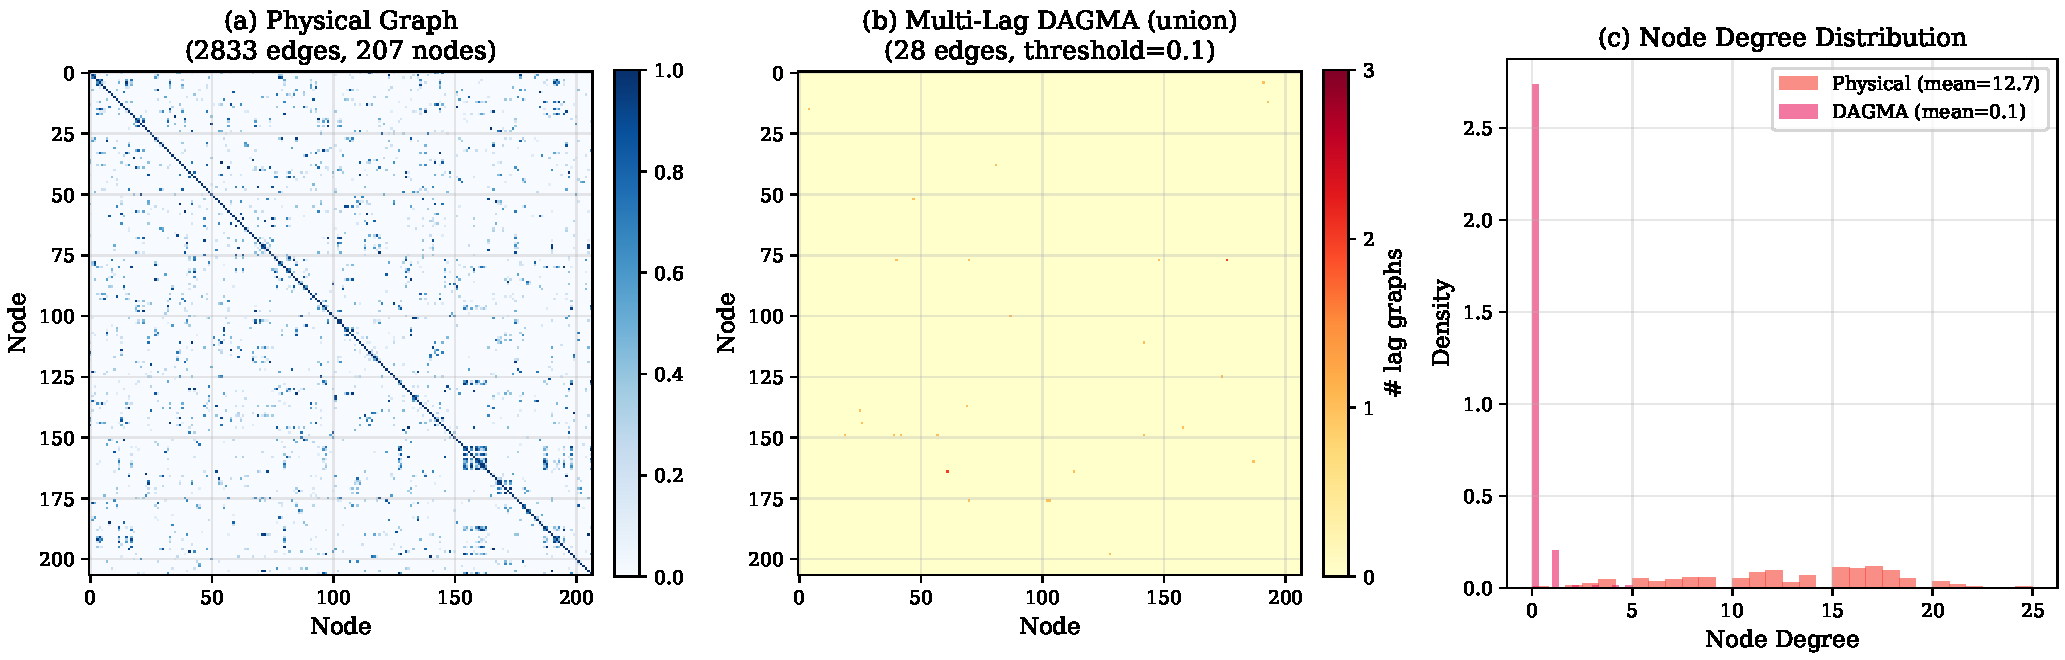
\includegraphics[width=0.95\textwidth]{figures/fig1_graph_comparison.pdf}
\caption{Physical versus learned graph structure (Los-loop). (a) Physical adjacency matrix with 2833 edges. (b) Multi-lag DAGMA union graph with 30 edges ($\tau=0.1$). (c) Node degree distribution: physical graph has mean degree 12.7, while DAGMA graph has mean degree 0.14.}
\label{fig:graph_comparison}
\end{figure}

\subsection{From Single-Graph GSL to Multi-Lag Structure}\label{sec:multilag_structure}

The original submission's GSL/cGSL experiments (Appendix~\ref{app:original_gsl}) established that a sparse DAGMA-learned graph substantially outperforms the dense physical adjacency for both GCN and T-GCN, with a striking asymmetry: the symmetrized cyclic variant (cGSL) was optimal for the purely spatial GCN, while the acyclic DAG was optimal for the temporally equipped T-GCN. On Los-loop, TGCN-GSL reduced RMSE by a mean 21.8\% across horizons PH=1--4 relative to the physical graph (e.g., PH=1: 6.588 $\rightarrow$ 4.818), a single-seed result whose full tables and protocol are retained in Appendix~\ref{app:original_gsl}. That asymmetry raised the question this revision answers: \emph{what does a single learned DAG actually encode?} Two controls were missing in the original study. First, a no-graph baseline, which reveals that the dense physical graph itself is harmful (Section~\ref{sec:oversmoothing}). Second, an explicit temporal decomposition of the learned structure, which the multi-lag formulation provides---converting a post-hoc interpretation of one ambiguous matrix into directly measurable, structurally distinct lag-specific graphs.

The multi-lag DAGMA formulation ($L=3$) produces lag-specific graphs with substantially different structures. Table~\ref{tab:lag_stats} reports the statistics for Los-loop at threshold $\tau = 0.1$.

\begin{table}[t]
\centering
\caption{Multi-lag DAGMA block statistics (Los-loop, $L=3$, $\tau=0.1$). Different lag blocks capture different dependency structures. Edge counts include self-loops; the corresponding cross-sensor training graphs (self-loops removed) retain 12, 3, and 15 edges for lag\_1, lag\_2, and lag\_3 respectively (30 in total).}
\label{tab:lag_stats}
\begin{tabular}{lcccc}
\toprule
\textbf{Block} & \textbf{Interpretation} & \textbf{Edges} & \textbf{Max $|w|$} & \textbf{Density} \\
\midrule
current & $x(t) \rightarrow x(t)$ & 70 & 0.653 & 0.001634 \\
lag\_1 & $x(t{-}1) \rightarrow x(t)$ & 90 & 0.804 & 0.002100 \\
lag\_2 & $x(t{-}2) \rightarrow x(t)$ & 5 & 0.673 & 0.000117 \\
lag\_3 & $x(t{-}3) \rightarrow x(t)$ & 16 & 0.296 & 0.000373 \\
\bottomrule
\end{tabular}
\end{table}

The current block has 70 cross-sensor edges, lag\_1 has 90 edges (dominated by self-loops), lag\_2 has only 5 edges, and lag\_3 has 16 edges. These blocks are structurally distinct, confirming that traffic dependencies are temporally heterogeneous.

\begin{figure}[t]
\centering

\includegraphics[width=\textwidth]{figures/fig7_lag_edge_stats.pdf}
\caption{Lag-specific graph analysis. (a) Edge count per lag for Los-loop and SZ-Taxi ($\tau=0.1$). (b) Jaccard overlap between lag-specific edge sets (Los-loop): low overlap confirms structural distinctness. (c) DAGMA weight distributions per lag.}
\label{fig:lag_stats}
\end{figure}

\subsection{T-GCN-MultiGSL-Mix: Multi-Seed Validation and Parameter Control}\label{sec:multiseed}\label{sec:param_control}

Table~\ref{tab:multiseed} presents the primary result: Los-loop, PH=1, five random seeds.

\begin{table}[t]
\centering
\caption{Multi-seed validation on Los-loop (PH=1). T-GCN-MultiGSL-Mix outperforms T-GCN-NoSpatial in all five seeds. Mean improvement: 14.9\%.}
\label{tab:multiseed}
\begin{tabular}{lcccccc}
\toprule
\textbf{Method} & \textbf{S42} & \textbf{S43} & \textbf{S44} & \textbf{S45} & \textbf{S46} & \textbf{Mean$\pm$Std} \\
\midrule
T-GCN-NoSpatial & 5.143 & 5.281 & 5.386 & 5.205 & 5.154 & 5.234$\pm$0.090 \\
T-GCN-MultiGSL & 4.717 & 4.737 & 4.752 & 4.994 & 4.771 & 4.794$\pm$0.102 \\
\textbf{T-GCN-MultiGSL-Mix} & \textbf{4.458} & \textbf{4.660} & \textbf{4.335} & \textbf{4.261} & \textbf{4.547} & \textbf{4.452$\pm$0.143} \\
\bottomrule
\end{tabular}
\end{table}

T-GCN-MultiGSL-Mix beats T-GCN-NoSpatial in all 5 seeds with a mean RMSE of 4.452 versus 5.234, corresponding to a 14.9\% improvement (five-seed mean; the seed-42-only comparison is 13.3\%). The fixed multi-graph approach also consistently outperforms T-GCN-NoSpatial (8.4\% improvement), but T-GCN-MultiGSL-Mix provides an additional 7.1\% improvement through learned graph mixing.

\begin{figure}[t]
\centering

\includegraphics[width=0.9\textwidth]{figures/fig3_multiseed_boxplot.pdf}
\caption{Multi-seed validation on Los-loop (PH=1, seeds 42--46). (a) Box plot: T-GCN-MultiGSL-Mix consistently outperforms T-GCN-NoSpatial across all seeds. (b) Mean RMSE $\pm$ std: T-GCN-MultiGSL-Mix achieves 4.452$\pm$0.143 versus T-GCN-NoSpatial 5.234$\pm$0.090 (14.9\% improvement).}
\label{fig:multiseed}
\end{figure}

To rule out the explanation that T-GCN-MultiGSL-Mix's improvement comes from having more parameters, we compare against a T-GCN-NoSpatial with matched capacity (Table~\ref{tab:param_control}).

\begin{table}[t]
\centering
\caption{Parameter-matched control (Los-loop, PH=1, seed=42). Adding 35\% more parameters to T-GCN-NoSpatial improves RMSE by only 0.1\%. T-GCN-MultiGSL-Mix's improvement is from the gating architecture.}
\label{tab:param_control}
\begin{tabular}{lccc}
\toprule
\textbf{Model} & \textbf{hidden\_dim} & \textbf{Parameters} & \textbf{RMSE} \\
\midrule
T-GCN-NoSpatial & 64 & 12,672 & 5.143 \\
T-GCN-NoSpatial (larger) & 74 & 16,872 & 5.137 \\
\textbf{T-GCN-MultiGSL-Mix} & 64 & \textbf{17,091} & \textbf{4.458} \\
\bottomrule
\end{tabular}
\end{table}

The parameter-matched T-GCN-NoSpatial (16,872 parameters) achieves RMSE 5.137, virtually identical to the standard T-GCN-NoSpatial (5.143). T-GCN-MultiGSL-Mix (17,091 parameters) achieves 4.458. Thus 99\% of the improvement comes from the gating architecture, not from additional capacity.

\paragraph{Predicted vs.\ actual behaviour.}
Figure~\ref{fig:pred_vs_actual} shows one-step-ahead predictions for the three most variable Los-loop nodes over a 100-step test window (PH=1, seed=42). Both models follow the ground truth closely---the overall Pearson correlation between predictions and observations across the full test set is $r=0.95$ for T-GCN-MultiGSL-Mix and $r=0.93$ for T-GCN-NoSpatial, with per-node values reaching $r\approx0.99$---and both exhibit the smooth, slightly lagged character typical of MSE-trained predictors that approximate conditional means. On two of the three displayed nodes, T-GCN-MultiGSL-Mix tracks rapid changes more faithfully than T-GCN-NoSpatial (windowed $r$ of 0.95 vs.\ 0.92 and 0.96 vs.\ 0.94), consistent with its lower RMSE; the remaining node is a low-signal case on which both models correlate weakly with the truth.

\begin{figure}[t]
\centering

\includegraphics[width=0.85\textwidth]{figures/fig9_predicted_vs_actual.pdf}
\caption{Predicted vs.\ actual traffic speed for three high-variance nodes on Los-loop (PH=1, seed=42), 100 consecutive test steps. Both T-GCN-NoSpatial and T-GCN-MultiGSL-Mix predictions closely track the ground truth, with the smooth, slightly lagged character typical of MSE-trained models. Per-node windowed correlations are given in the text.}
\label{fig:pred_vs_actual}
\end{figure}

\subsection{Ablation: Lags and Prediction Horizons}\label{sec:lag_ablation}

Table~\ref{tab:lag_ablation} shows the contribution of each temporal lag.

\begin{table}[t]
\centering
\caption{Lag ablation (Los-loop, PH=1, seed=42). All three lags contribute; the full combination is best.}
\label{tab:lag_ablation}
\begin{tabular}{lccc}
\toprule
\textbf{Configuration} & \textbf{Edges} & \textbf{RMSE} & \textbf{Improvement} \\
\midrule
T-GCN-NoSpatial & 207 & 5.143 & --- \\
lag\_2 only & 3 & 4.619 & 10.2\% \\
lag\_3 only & 15 & 4.605 & 10.5\% \\
lag\_1 only & 12 & 4.605 & 10.5\% \\
lag\_1+lag\_3 & 27 & 4.646 & 9.7\% \\
lag\_2+lag\_3 & 18 & 4.638 & 9.8\% \\
lag\_1+lag\_2 & 15 & 4.559 & 11.4\% \\
\textbf{All 3 lags} & \textbf{30} & \textbf{4.458} & \textbf{13.3\%} \\
\bottomrule
\end{tabular}
\end{table}

Each individual lag provides approximately 10\% improvement over T-GCN-NoSpatial. The best two-lag combination is lag\_1+lag\_2 (11.4\%), and the full three-lag configuration achieves 13.3\%. This confirms that all three temporal scales carry complementary predictive information.

\begin{figure}[t]
\centering

\includegraphics[width=0.9\textwidth]{figures/fig5_lag_ablation.pdf}
\caption{Lag ablation study (Los-loop, PH=1, seed=42). Each lag provides $\sim$10\% improvement individually; all three lags together achieve 13.3\%. Color intensity reflects number of lags used.}
\label{fig:lag_ablation}
\end{figure}

Table~\ref{tab:multiph} reports results across all four prediction horizons on Los-loop.

\begin{table}[t]
\centering
\caption{Multi-horizon results on Los-loop (seed=42). T-GCN-MultiGSL-Mix consistently outperforms T-GCN-NoSpatial and Physical across all horizons.}
\label{tab:multiph}
\begin{tabular}{lcccc}
\toprule
\textbf{Method} & \textbf{PH=1} & \textbf{PH=2} & \textbf{PH=3} & \textbf{PH=4} \\
\midrule
Physical & 7.658 & 8.002 & 8.512 & 8.540 \\
T-GCN-NoSpatial & 5.143 & 5.642 & 6.164 & 6.502 \\
T-GCN-MultiGSL & 4.715 & 5.549 & 5.934 & 6.336 \\
\textbf{T-GCN-MultiGSL-Mix} & \textbf{4.458} & \textbf{5.308} & \textbf{5.687} & \textbf{6.004} \\
\bottomrule
\end{tabular}
\end{table}

On Los-loop, T-GCN-MultiGSL-Mix consistently outperforms T-GCN-NoSpatial across all horizons, with the largest relative improvement at PH=1 (13.3\%). The advantage persists but narrows at longer horizons. The dependence of performance on the DAGMA threshold $\tau$---and hence on the learned sparsity level---is reported in Appendix~\ref{app:diagnostics}: T-GCN-MultiGSL-Mix achieves its best RMSE near the operating point of 30 edges.

\subsection{Robustness Across Temporal Resolution}\label{sec:los15min}

Does the effect survive a change of sampling interval on the same sensor network? We resample Los-loop to 15-minute intervals (three-step averaging, $T=672$) and repeat the full pipeline---DAGMA learned once on the 15-minute training split, then reused across horizons. Table~\ref{tab:los15min} reports five-seed results.

\begin{table}[t]
\centering
\caption{Los-loop at 15-minute sampling (seeds 42--46, mean$\pm$std). PH=$k$ denotes $k\times15$ minutes ahead: 15, 30, 45, and 60 minutes for $k=1$--4. RMSE magnitudes are not directly comparable with the 5-minute tables above, so we compare relative improvements. The lag graphs (32 cross-sensor edges over three lags) come from a single PH-independent DAGMA run on the 15-minute training split.}
\label{tab:los15min}
\small
\setlength{\tabcolsep}{4pt}
\begin{tabular}{lcccc}
\toprule
\textbf{Method} & \textbf{PH=1} & \textbf{PH=2} & \textbf{PH=3} & \textbf{PH=4} \\
\midrule
T-GCN-NoSpatial & 8.600$\pm$0.249 & 9.311$\pm$0.197 & 10.048$\pm$0.074 & 10.460$\pm$0.196 \\
T-GCN-MultiGSL & 7.246$\pm$0.298 & 8.571$\pm$0.327 & 9.112$\pm$0.077 & 9.756$\pm$0.210 \\
\textbf{T-GCN-MultiGSL-Mix} & \textbf{6.240$\pm$0.187} & \textbf{7.322$\pm$0.338} & \textbf{8.063$\pm$0.203} & \textbf{8.777$\pm$0.326} \\
\midrule
\textbf{Mix improvement} & \textbf{+27.4\%} & +21.4\% & +19.8\% & +16.1\% \\
\bottomrule
\end{tabular}
\end{table}

At 15-minute sampling the relative improvement over T-GCN-NoSpatial is \emph{larger} than at 5-minute sampling: +27.4\% at PH=1 versus +14.9\% (five-seed mean), with T-GCN-MultiGSL-Mix winning in all five seeds (per-seed improvements of +23.2\% to +31.3\%) and the advantage persisting across all four horizons. This shows that the multi-lag benefit is not an artifact of one sampling interval; the implications for the dataset-dependence analysis below are discussed in Section~\ref{sec:discussion}.

\subsection{Dataset Dependence: the SZ-Taxi Boundary}\label{sec:sz_boundary}

Table~\ref{tab:sz_multiph} reports the SZ-Taxi results, promoted here from the appendix because the boundary of the method is as informative as its successes.

\begin{table}[t]
\centering
\caption{SZ-Taxi multi-horizon results (seed=42, single seed). T-GCN-MultiGSL-Mix improvement is marginal. Note that the oversmoothing pattern replicates: the dense physical graph is again far worse than no graph.}
\label{tab:sz_multiph}
\begin{tabular}{lcccc}
\toprule
\textbf{Method} & \textbf{PH=1} & \textbf{PH=2} & \textbf{PH=3} & \textbf{PH=4} \\
\midrule
Physical & 5.267 & 5.406 & 5.629 & 5.604 \\
T-GCN-NoSpatial & 4.116 & 4.160 & 4.189 & 4.221 \\
\textbf{T-GCN-MultiGSL-Mix} & 4.108 & 4.149 & 4.184 & 4.221 \\
\bottomrule
\end{tabular}
\end{table}

On SZ-Taxi the improvement is marginal: $\leq0.3\%$ at PH=1--3 and $-0.02\%$ at PH=4 (single seed). This is not explained by temporal resolution: SZ-Taxi and the 15-minute Los-loop variant share the sampling interval, yet Los-loop shows strong improvements at both 5-minute and 15-minute sampling (Sections~\ref{sec:multiseed} and~\ref{sec:los15min}), so the divergence tracks the dataset rather than the sampling interval. A candidate mechanism consistent with the evidence is graph learnability: at the operating threshold, DAGMA retains only 2 cross-sensor edges for SZ-Taxi versus 30--32 for Los-loop, suggesting that the urban network's dependency structure at 15-minute aggregation offers the learner far less exploitable signal. Other dataset differences (156 vs.\ 207 sensors, urban vs.\ highway dynamics) may also contribute. We therefore report SZ-Taxi as a dataset-dependent boundary of the method rather than claiming universal benefit.
